\documentclass{article}
\usepackage[utf8]{inputenc}
\usepackage{tikz}
\usetikzlibrary{shapes.geometric, arrows}

%\tikzstyle{startstop} = [rectangle, rounded corners, minimum width=3cm, minimum height=1cm,text centered, draw=black, fill=red!30]
%\tikzstyle{io} = [trapezium, trapezium left angle=70, trapezium right angle=110, minimum width=3cm, minimum height=1cm, text centered, draw=black, fill=blue!30]
%\tikzstyle{process} = [rectangle, minimum width=3cm, minimum height=1cm, text centered, text width=3cm, draw=black, fill=orange!30]
%\tikzstyle{decision} = [diamond, minimum width=3cm, minimum height=1cm, text centered, draw=black, fill=green!30]
%\tikzstyle{arrow} = [thick,->,>=stealth]
\tikzstyle{decision} = [ diamond, draw, fill=blue!20, text width=4.5em, text badly centered, node distance=3cm, inner sep-0pt]  
\tikzstyle{block} = [ rectangle, draw, fill=blue!20, text width=5em, text badly centered, rounded corners, minimum height=4em]  
\tikzstyle{line} = [ draw, -latex']  
\tikzstyle{terminator} = [ draw, ellipse, fill=red!20, node distance=3cm, minimum height=2em]  

\begin{document}

%\begin{tikzpicture}[node distance=2cm]
%
%\node (start) [startstop] {Choose the frequency of the input signal};
%\node (in1) [io, below of=start] {Compute the period for the ADC and DAC associated (using Eq 1)};
%\node (pro1) [process, below of=in1] {Make a call to 'pay\_conf\_expFis' with the period calculated} ;
%\node (pro2) [process, below of=pro1] {Configure the Timer4 and Timer5 to trigger the DAC/ADC};
%\node (pro3) [process, below of=pro2, yshift=-0.75cm] {Make a call to 'pay\_exec\_expFis'};
%\node (dec1) [decision, below of=pro3, yshift=-0.75cm] {finished?};
%\node (pro2a) [process, right of=dec1, xshift=3cm] {Wait until finishes};
%\node (pro2b) [process, below of=dec1, yshift=-0.75cm] {Parse count values to voltages};
%\node (out1) [io, below of=pro2b] {Output};
%\node (stop) [startstop, below of=out1] {Stop};
%
%\draw [arrow] (start) -- (in1);
%\draw [arrow] (in1) -- (pro1);
%\draw [arrow] (pro1) -- (pro2);
%\draw [arrow] (pro2) -- (pro3);
%\draw [arrow] (pro3) -- (dec1);
%\draw [arrow] (dec1) -- node[anchor=south] {yes} (pro2b);
%\draw [arrow] (dec1) -- node[anchor=east] {no} (dec1);
%\draw [arrow] (pro2b) -- (out1);
%\draw [arrow] (out1) -- (stop);
%\end{tikzpicture}

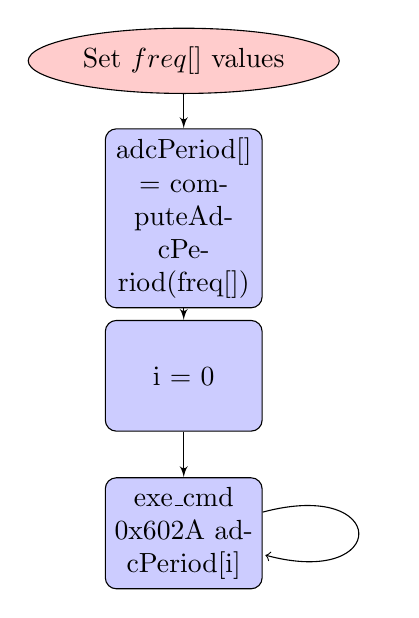
\begin{tikzpicture}[node distance=2cm, auto]  
  \node [terminator]           (puc)  {Set $freq[]$ values};  
  \node [block, below of=puc]  (wdt)  {adcPeriod[] = computeAdcPeriod(freq[])};  
  \node [block, below of=wdt]  (port) {i = 0};  
  \node [block, below of=port] (loop) {exe\_cmd 0x602A adcPeriod[i]};  
  \path [line] (puc)  -- (wdt);  
  \path [line] (wdt)  -- (port);  
  \path [line] (port) -- (loop);  
 % \path [line] (loop) -- (loop);  
  \path [line] (loop) edge[loop right]();
\end{tikzpicture}


\end{document}
